\documentclass[../mathNotesPreamble]{subfiles}
\begin{document}
%\relscale{1.4} %TODO
\section{16.7: Change of Variables in Multiple Integrals}


\noindent Recall in Calculus I that the Substitution Rule allow us to perform a \textit{change of variables}. Reversing the order, if we set $x=g(u)$ and $dx=g'(u)du$,
\[
\int_{g(c)}^{g(d)} f\parens{x}~dx\overset{\text{sub}}{=}\int_{c}^{d}f\parens{g(u)}g'(u)~du
\]
\noindent In Sections 16.3 and 16.5, we used a change of variables to rewrite our integrals in terms of polar curves (2D) and cylindrical/spherical (3D). What if we want to change our current coordinate system to \textit{any} coordinate system?\\

\noindent\textbf{Change of Coordinates in 2D}
\begin{defn*}[Jacobian]
Suppose $x=g(u,v)$ and $y=h(u,v)$ represent a transformation from the $uv-$coordinate system to $xy-$coordinate system. The \textbf{Jacobian} of this transformation is 
\[
J(u,v)=\dfrac{\partial\parens{x,y}}{\partial\parens{u,v}}=\begin{vmatrix}
\dfrac{\partial x}{\partial u}&\dfrac{\partial x}{\partial v}\\[2ex]
\dfrac{\partial y}{\partial u}&\dfrac{\partial y}{\partial v}
\end{vmatrix}=\dfrac{\partial x}{\partial u}\dfrac{\partial y}{\partial v}-\dfrac{\partial y}{\partial u}\dfrac{\partial x}{\partial v}
\]
\end{defn*}
\begin{ex*}
Compute the Jacobian for the transformation $x=r\cos\theta$ and $y=r\sin\theta$
\end{ex*}
\pagebreak
\begin{thmBox*}[Theorem 16.8: Change of Variables for Double Integrals]
Suppose that the transformation $x=g(u,v)$ and $y=g(u,v)$ has a nonzero Jacobian that maps a closed bounded region $S$ in the $uv-$plane to a region $R$ in the $xy-$plane. Let $f$ be a continuous function on $R$. Then
\[
\iint\limits_R f(x,y)~dA_1=\iint\limits_S f\parens{g(u,v),h(u,v)}
~\abs{J(u,v)}~dA_2\]
where $\abs{J(u,v)}$ denotes the absolute value of the Jacobian.
\end{thmBox*}
\begin{ex*}
Perform a change of variables for the integral $\displaystyle\iint_Rf(x,y)~dA$, where 
\[
R=\left\{\parens{r,\theta}: 0\leq a\leq r\leq b,\text{ }\alpha\leq\theta\beta\right\},\text{ }\beta-\alpha=2\pi
\] 
under the transformation $x=r\cos\theta$ and $y=r\sin\theta$.
\end{ex*}
\vspace*{\stretch{1}}
\pagebreak
\begin{ex*}
Let $R$ be the region bounded by the lines 
\[
x-2y=0,\text{ }x-2y=-4,\text{ }x+y=4,\text{ and }x+y=1.
\]
Evaluate the double integral $\displaystyle\iint\limits_R3xy~dA$.
\begin{flushleft}
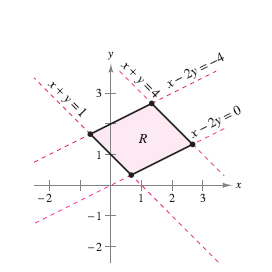
\includegraphics[width=.35\linewidth]{../images/briggs_16_07/fig16_420}
\end{flushleft}
\end{ex*}
  \pagebreak
  \begin{ex*}
  Let $R$ be the region in the first quadrant bounded by the parabolas $x=y^2$, $x=y^2-4$, $x=9-y^2$, and $x=16-y^2$. Evaluate $\displaystyle\iint\limits_R y^2~dA$
  \begin{flushleft}
  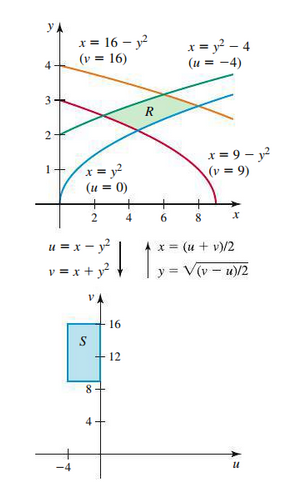
\includegraphics[width=.35\linewidth]{../images/briggs_16_07/fig16_22}
  \end{flushleft}
  \end{ex*}
  \pagebreak
  \begin{ex*}
  Evaluate the integral $\displaystyle\iint\limits_R e^{\sfrac{\parens{x+y}}{\parens{x-y}}}~dA$, where $R$ is the trapezodial region with vertices $(1,0)$, $(2,0)$, $(0,-2)$, and $(0,-1).$
\begin{flushleft}
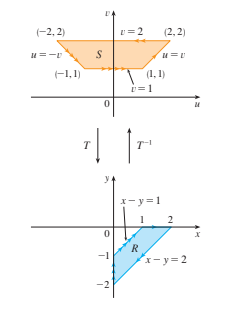
\includegraphics[width=.35\linewidth]{../images/briggs_16_07/fig16_21}
\end{flushleft}
  \end{ex*}
  \pagebreak
  \noindent\textbf{Change of Coordinates in 3D}\\
  
  \noindent We can perform a similar change of variables for triple integrals. For this change in variables, we make the appropriate adjustments from our current work.
  \begin{defn*}[Jacobian in 3D]
  Suppose $x=g(u,v,w)$, $y=h(u,v,w)$, and $z=p(u,v,w)$ represent a transformation from the $uvw-$coordinate system to $xyz-$coordinate system. The \textbf{Jacobian} of this transformation is
  \[
  J(u,v,w)=\dfrac{\partial(x,y,z)}{\partial(u,v,w)}=\begin{vmatrix}
  \dfrac{\partial x}{\partial u}& \dfrac{\partial x}{\partial v}& \dfrac{\partial x}{\partial w}\\[2ex]
   \dfrac{\partial y}{\partial u}& \dfrac{\partial y}{\partial v}& \dfrac{\partial y}{\partial u}\\[2ex]
    \dfrac{\partial z}{\partial u}& \dfrac{\partial z}{\partial v}& \dfrac{\partial z}{\partial w}\\
  \end{vmatrix}
  \]
  \end{defn*}
  \begin{thmBox*}[Theorem 16.9: Change of Variables for Triple Integrals]
Suppose that the transformation $x=g(u,v,w)$ and $y=g(u,v,w)$, and $z=p(u,v,w)$ has a nonzero Jacobian that maps a closed bounded region $S$ in the $uvw-$plane to a region $R$ in the $xyz-$plane. Let $f$ be a continuous function on $R$. Then
\[
\iiint\limits_R f(x,y,z)~dV_1=\iiint\limits_S f\parens{g(u,v,w),h(u,v,w),p(u,v,w)}
~\abs{J(u,v,w)}~dV_2\]
\end{thmBox*}
\noindent\textit{Note:} In Linear Algebra, the determinant of a matrix represents how much the volume of a region scales under a transformation. Thus, the Jacobian determines how much the volume scales, at a point, under the change of coordinates. This is why we multiply the integrand by the Jacobian, to account for the changes in volume between the two coordinate systems.
  \pagebreak
  \begin{ex*}
  Derive the formula for the triple integration in spherical coordinates.
  \end{ex*}
  \pagebreak
  \begin{ex*}
  Evaluate $\displaystyle\iiint\limits_Dxz~dV$, where $D$ is a parallelpiped bounded by the planes
  \[
  y=x,\text{ }y=x+2,\text{ }z=x,\text{ }z=x+3,\text{ }z=0,\text{ and }z=4
  \]
  \begin{flushleft}
  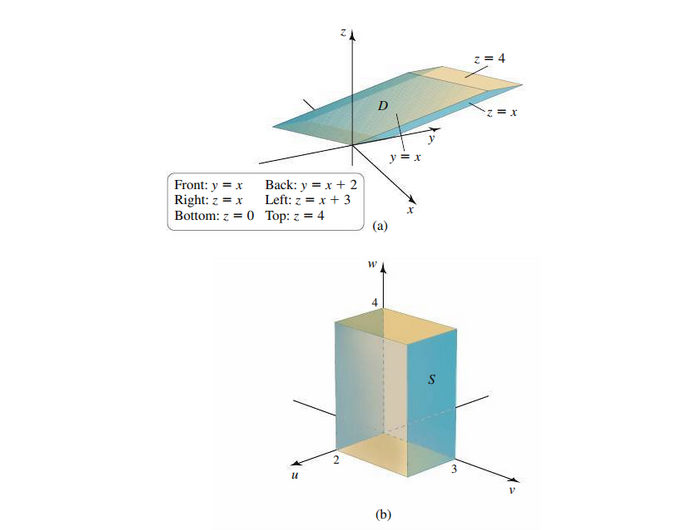
\includegraphics[width=.75\linewidth]{../images/briggs_16_07/fig16_83}
  \end{flushleft}
  \end{ex*}
  \pagebreak
  \noindent\textbf{Strategies for Choosing New Variables}\\

\noindent As when you learned the Substitution Rule for the first time, learning how to choose new variables for multiple integrals will be a bumpy road. Below is a guideline to aid you when you change variables. The guideline is made with respect to double integrals, but you can translate this to triple integrals as well:
\begin{enumerate}
\item\textbf{Aim for simple regions of integration in the $\emph{uv}-$plane:} One goal of changing the variables is to make the region you're integrating over as simple as possible. Hence, perform the transformation where  you make the new region straightforward to calculate. It would be ideal if you can transform the new region to a rectangular region.

\item\textbf{Determine the easier coordinate system:} You will encounter problems where it's easier to write $(x,y)$ as functions of $(u,v)$; in other problems, the opposite is true. 
\begin{itemize}
\item If you already know $(x,y)$ in terms of $(u,v)$, it's straightforward to get the Jacobian and sketching the region $R$. However, you must invert the transformation to determine the region $S$.

\item  If you already know $(u,v)$ in terms of $(x,y)$, knowing the region $S$ is straightforward. However, the transformation must be inverted to compute the Jacobian.
\end{itemize} 
\item\textbf{Take a hint from the integrand:} Sometimes the new variables are often chosen based on the integrand. Look for a composition appearing in the integrand and choose the inside functions. For example, if
\[
\sqrt{\dfrac{x-y}{x+y}}
\]
was the integrand of a double integral, choose the new variables $u=x-y$ and $v=x+y$.\\

If a combination of variables appears, let one new variable be the entire combination and set the other new variable as one of the original variables. For example, if the integrand of the double integral is $
\parens{x+4y}^{3/2}$
choose the new variables $u=x+4y$ and $v=y$.

\item\textbf{Take a hint from the given  region:} If you have a region that's bounded by two pairs of ``parallel" curves, you can transform the given region into a rectangular region. An illustration is provided below. In both regions, we can  transform them into the rectangle 
\[
S=\left\{(u,v):a_1\leq u\leq a_2,\text{ }b_1\leq v\leq b_2\right\}
\]
with $u=g(x,y)$ and $v=h(x,y).$
\begin{center}
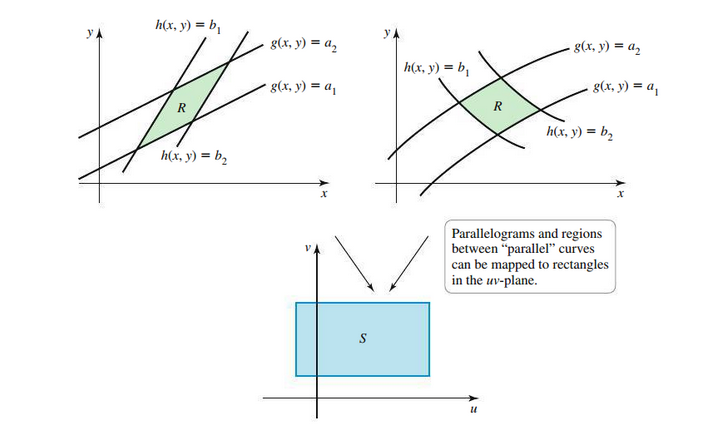
\includegraphics[width=\linewidth]{../images/briggs_16_07/fig16_84}
\end{center}
\end{enumerate}
  \pagebreak
\end{document}